% ==============================================================================
\chapter{Reduced Order Modeling (ROM) \& Hyper-Reduction}
\label{ch:rom}
% ==============================================================================

\begin{tcolorbox}[colback=lightbg, colframe=primaryblue, title=\textbf{Chapter at a Glance: Real-Time ROM \& Hyper-Reduction}, fonttitle=\bfseries]
\begin{description}[leftmargin=!, labelwidth=3.4cm]
    \item[\textbf{Core Strategy}] Project full displacement field onto low-dimensional POD basis $\boldsymbol{\Phi} \in \mathbb{R}^{N \times r}$ ($r = 15 \ll N = 6,564$).
    \item[\textbf{Hyper-Reduction}] Energy-Conserving Sampling and Weighting (ECSW) restricts integration loops to $E^* = 28$ active elements ($64.5\times$ speedup, $0.054\%$ error).
    \item[\textbf{Digital Twin}] Pure client-side JavaScript WebGL architecture running sub-millisecond solves ($<1.5\,\text{ms}$) at interactive frame rates ($\ge 20\,\text{FPS}$).
\end{description}
\end{tcolorbox}

% ------------------------------------------------------------------------------
\section{The Model Reduction Strategy \& 5-Step Recipe}
% ------------------------------------------------------------------------------

To achieve sub-millisecond solves for interactive WebGL Digital Twins without sacrificing physical accuracy ($L_2$ error $<0.1\%$), we implement a 5-step offline/online projection recipe:

\begin{tcolorbox}[colback=lightbg, colframe=primaryblue, title={\textbf{Step 1: Pullback Mapping to Static Reference Domain $\hat{\Omega}$}}, fonttitle=\bfseries]
Pull back weak form integrals from $\Omega(\boldsymbol{\mu})$ to $\hat{\Omega}$ to ensure snapshot vectors and bases reside in an invariant vector space $\mathbb{R}^N$.
\end{tcolorbox}

\begin{tcolorbox}[colback=lightbg, colframe=primaryblue, title={\textbf{Step 2: Offline Snapshot Collection (Data Generation)}}, fonttitle=\bfseries]
Execute high-fidelity FOM sweeps across parameters $\boldsymbol{\mu} = (x_c, r)^T \in \mathcal{D}$, assembling displacement fields into snapshot matrix $\mathbf{S}_u$.
\end{tcolorbox}

\begin{tcolorbox}[colback=lightbg, colframe=primaryblue, title={\textbf{Step 3: Proper Orthogonal Decomposition (POD Basis Construction)}}, fonttitle=\bfseries]
Perform SVD on $\mathbf{S}_u = \mathbf{U} \boldsymbol{\Sigma} \mathbf{V}^T$ to extract dominant modes $\boldsymbol{\Phi} \in \mathbb{R}^{N \times r}$ capturing $\ge 99.999\%$ modal energy.
\end{tcolorbox}

\begin{tcolorbox}[colback=lightbg, colframe=primaryblue, title={\textbf{Step 4: Hyper-Reduction Training (ECSW NNLS Optimization)}}, fonttitle=\bfseries]
Solve Non-Negative Least Squares (NNLS) to select a minimal subset of active elements $E^* \subset E$ ($E^*=28$) and positive integration weights $w_e$.
\end{tcolorbox}

\begin{tcolorbox}[colback=lightbg, colframe=primaryblue, title={\textbf{Step 5: Real-Time Online Interactive Simulation}}, fonttitle=\bfseries]
Execute reduced $r \times r$ integration loops over $E^*$ in JavaScript, maintaining transient state projection across parameter slider updates.
\end{tcolorbox}

% ------------------------------------------------------------------------------
\section{Standard Galerkin ROM \& POD Basis Truncation}
\label{sec:galerkin_rom}
% ------------------------------------------------------------------------------

The high-fidelity displacement vector $\vect{U}(t) \in \mathbb{R}^N$ is projected onto the Reduced Basis matrix $\boldsymbol{\Phi} \in \mathbb{R}^{N \times r}$ ($r \ll N$):
\begin{equation}
    \vect{U}(t) \approx \boldsymbol{\Phi} \vect{q}(t)
\end{equation}

Cumulative modal energy fraction $\eta(r)$ and relative $L_2$ projection error $\epsilon(r)$ are defined as:
\begin{equation}
    \eta(r) = \frac{\sum_{i=1}^{r} \sigma_i^2}{\sum_{j=1}^{d} \sigma_j^2}, \quad \epsilon(r) = \sqrt{1 - \eta(r)}
\end{equation}

Figure \ref{fig:pod_energy_decay} illustrates the rapid spectral convergence of singular values, confirming that $r = 15$ modes capture $99.999\%$ of total system energy.

\begin{figure}[htbp]
    \centering
    \begin{subfigure}{0.48\textwidth}
        \centering
        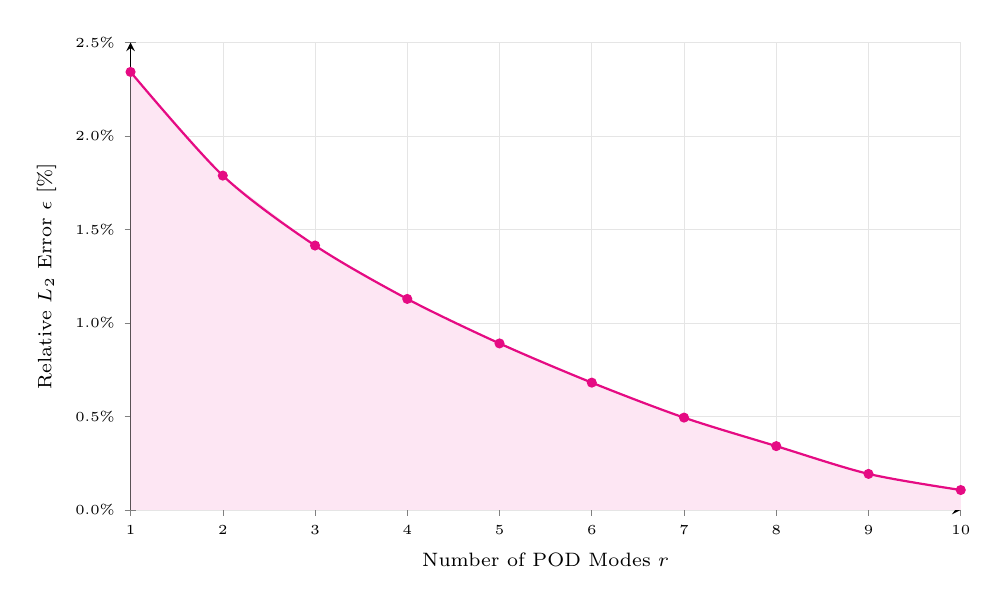
\begin{tikzpicture}
            \begin{axis}[
                width=1.0\textwidth,
                height=0.62\textwidth,
                xlabel={Number of POD Modes $r$},
                ylabel={Relative $L_2$ Error $\epsilon$ [\%]},
                xmin=1, xmax=10,
                ymin=0, ymax=2.5,
                xtick={1,2,3,4,5,6,7,8,9,10},
                ytick={0, 0.5, 1.0, 1.5, 2.0, 2.5},
                yticklabels={0.0\%, 0.5\%, 1.0\%, 1.5\%, 2.0\%, 2.5\%},
                grid=both,
                grid style={line width=.1pt, draw=gray!10},
                major grid style={line width=.2pt, draw=gray!20},
                axis lines=left,
                enlargelimits=false,
                x tick label style={font=\tiny},
                y tick label style={font=\tiny},
                xlabel style={font=\scriptsize},
                ylabel style={font=\scriptsize},
            ]
                \addplot[fill=magenta!10, draw=none] coordinates {
                    (1, 2.3424) (2, 1.7880) (3, 1.4139) (4, 1.1283) (5, 0.8902)
                    (6, 0.6806) (7, 0.4935) (8, 0.3410) (9, 0.1924) (10, 0.1062)
                } \closedcycle;
                \addplot[color=magenta!85!purple, mark=*, thick, smooth, mark options={fill=magenta!85!purple, scale=0.7}] coordinates {
                    (1, 2.3424) (2, 1.7880) (3, 1.4139) (4, 1.1283) (5, 0.8902)
                    (6, 0.6806) (7, 0.4935) (8, 0.3410) (9, 0.1924) (10, 0.1062)
                };
            \end{axis}
        \end{tikzpicture}
        \caption{Relative $L_2$ projection error $\epsilon(r)$.}
    \end{subfigure}
    \hfill
    \begin{subfigure}{0.48\textwidth}
        \centering
        \begin{tikzpicture}
            \begin{axis}[
                width=1.0\textwidth,
                height=0.62\textwidth,
                xlabel={Number of POD Modes $r$},
                ylabel={Cumulative Energy $\eta$ [\%]},
                xmin=1, xmax=10,
                ymin=99.9, ymax=100.0,
                xtick={1,2,3,4,5,6,7,8,9,10},
                ytick={99.9, 99.92, 99.94, 99.96, 99.98, 100.0},
                yticklabels={99.90\%, 99.92\%, 99.94\%, 99.96\%, 99.98\%, 100.00\%},
                grid=both,
                grid style={line width=.1pt, draw=gray!10},
                major grid style={line width=.2pt, draw=gray!20},
                axis lines=left,
                enlargelimits=false,
                x tick label style={font=\tiny},
                y tick label style={font=\tiny},
                xlabel style={font=\scriptsize},
                ylabel style={font=\scriptsize},
            ]
                \addplot[fill=accentcyan!15, draw=none] coordinates {
                    (1, 99.9451) (2, 99.9680) (3, 99.9800) (4, 99.9873) (5, 99.9921)
                    (6, 99.9954) (7, 99.9976) (8, 99.9988) (9, 99.9996) (10, 99.9999)
                } \closedcycle;
                \addplot[color=primaryblue, mark=*, thick, smooth, mark options={fill=primaryblue, scale=0.7}] coordinates {
                    (1, 99.9451) (2, 99.9680) (3, 99.9800) (4, 99.9873) (5, 99.9921)
                    (6, 99.9954) (7, 99.9976) (8, 99.9988) (9, 99.9996) (10, 99.9999)
                };
            \end{axis}
        \end{tikzpicture}
        \caption{Cumulative modal energy fraction $\eta(r)$.}
    \end{subfigure}
    \caption{Proper Orthogonal Decomposition (POD) spectral convergence analysis showing relative projection error decay (left) and cumulative energy fraction (right).}
    \label{fig:pod_energy_decay}
\end{figure}

Applying Galerkin projection yields the $r \times r$ reduced dynamic system:
\begin{equation}
    \mathbf{M}_r \ddot{\vect{q}}(t) + \mathbf{C}_r \dot{\vect{q}}(t) + \mathbf{K}_r(\boldsymbol{\mu}) \vect{q}(t) = \mathbf{F}_r(t)
\end{equation}
where the projected operators are defined as:
\begin{equation}
    \mathbf{M}_r = \boldsymbol{\Phi}^T \hat{\mathbf{M}} \boldsymbol{\Phi}, \quad \mathbf{K}_r(\boldsymbol{\mu}) = \boldsymbol{\Phi}^T \hat{\mathbf{K}}(\boldsymbol{\mu}) \boldsymbol{\Phi}, \quad \mathbf{C}_r = \boldsymbol{\Phi}^T \hat{\mathbf{C}} \boldsymbol{\Phi}, \quad \mathbf{F}_r(t) = \boldsymbol{\Phi}^T \hat{\mathbf{F}}_{\text{ext}}(t)
\end{equation}

For very low-dimensional systems ($r=2$), the linear system $\mat{K}_{\text{eff},r}\Delta \vect{q} = \vect{R}_r$ is solved analytically via Cramer's Rule:
\begin{equation}
    \Delta q_1 = \frac{R_1 K_{22} - R_2 K_{12}}{\det(\mathbf{K}_{\text{eff}, r})}, \quad \Delta q_2 = \frac{K_{11} R_2 - K_{21} R_1}{\det(\mathbf{K}_{\text{eff}, r})}
\end{equation}

Table \ref{tab:mapping_tradeoffs} summarizes the algorithmic trade-offs of reference configuration mapping.

\begin{table}[htbp]
    \centering
    \caption{Algorithmic trade-offs of the reference configuration mapping paradigm.}
    \label{tab:mapping_tradeoffs}
    \resizebox{\textwidth}{!}{%
    \begin{tabular}{p{7.5cm} p{7.5cm}}
        \toprule
        \textbf{Advantages} & \textbf{Drawbacks} \\
        \midrule
        \textbf{1. Single Mesh Topology}: Reference domain $\hat{\Omega}$ is discretized once without mesh distortion. & \textbf{1. Algebraic Complexity}: Introduces parameter-dependent Jacobians $\mathbf{J}_{\hat{\vect{x}}}^{-T}(\boldsymbol{\mu})$ and $J_{\hat{\vect{x}}, \boldsymbol{\mu}}$. \\
        \textbf{2. Static Basis Functions}: NURBS basis $\hat{R}_i(\boldsymbol{\xi})$ is parameter-independent, enabling SVD snapshot matrices. & \textbf{2. Push-Forward Visual Field}: Spatial displacement field must be pushed forward to physical space $\Omega(\boldsymbol{\mu})$ for WebGL display. \\
        \textbf{3. Affine Precomputability}: Static spatial terms pre-evaluated offline. & \\
        \bottomrule
    \end{tabular}%
    }
\end{table}

\begin{figure}[htbp]
    \centering
    \begin{tikzpicture}[scale=1.1, >=stealth]
        % LEFT PANEL: Parameterized Physical Domain \Omega(\mu)
        \begin{scope}[xshift=-4.5cm, yshift=0cm, scale=0.85]
            \node[above=0.5cm, font=\small\bfseries\sffamily, text=primaryblue] at (2.5, 0.8) {Physical Domain $\Omega(\boldsymbol{\mu})$};
            % Clamped support
            \draw[line width=1.5pt] (0,0.8) -- (0,-0.8);
            \foreach \y in {-0.7,-0.4,...,0.7} {
                \draw (0,\y) -- (-0.2,\y-0.12);
            }
            % Notched deformed beam outline
            \shade[left color=primaryblue!25, right color=accentcyan!20, draw=primaryblue, thick]
            (0, 0.8) -- (1.6, 0.8) .. controls (2.1, 0.8) and (2.3, 0.25) .. (2.6, 0.25)
            .. controls (2.9, 0.25) and (3.1, 0.8) .. (3.6, 0.8) -- (5.0, 0.8) -- (5.0, -0.8) -- (3.6, -0.8)
            .. controls (3.1, -0.8) and (2.9, -0.25) .. (2.6, -0.25)
            .. controls (2.3, -0.25) and (2.1, -0.8) .. (1.6, -0.8) -- (0, -0.8) -- cycle;
            
            % Deformed curvilinear grid lines
            \foreach \x in {1.0, 2.0, 3.0, 4.0} {
                \draw[primaryblue!40, thin] (\x, -0.7) -- (\x, 0.7);
            }
            \draw[primaryblue!40, thin] (0, 0) -- (5.0, 0);
            \node[font=\small\bfseries, primaryblue] at (2.6, 0) {$\vect{x} \in \Omega(\boldsymbol{\mu})$};
            \node[font=\small, text=black!70] at (2.5, -1.2) {Notched Geometry $\boldsymbol{\mu} = (x_c, r)$};
        \end{scope}

        % CENTER ARROW: Bijective Pullback Diffeomorphism (Clean Gap between beams)
        \draw[<->, ultra thick, primaryblue] (-0.1, 0) -- (0.7, 0) 
            node[midway, above=3pt, font=\small\bfseries] {$\boldsymbol{\Psi}(\hat{\vect{x}}; \boldsymbol{\mu})$} 
            node[midway, below=3pt, font=\small, text=black!70] {Bijective Pullback};

        % RIGHT PANEL: Static Rectangular Reference Domain \hat{\Omega}
        \begin{scope}[xshift=0.9cm, yshift=0cm, scale=0.85]
            \node[above=0.5cm, font=\small\bfseries\sffamily, text=black!85] at (2.5, 0.8) {Static Reference Domain $\hat{\Omega}$};
            % Clamped support
            \draw[line width=1.5pt] (0,0.8) -- (0,-0.8);
            \foreach \y in {-0.7,-0.4,...,0.7} {
                \draw (0,\y) -- (-0.2,\y-0.12);
            }
            % Flat rectangular reference beam outline
            \shade[left color=gray!25, right color=gray!10, draw=black!70, thick]
            (0, -0.8) rectangle (5.0, 0.8);
            
            % Flat invariant reference grid
            \foreach \x in {1.0, 2.0, 3.0, 4.0} {
                \draw[black!30, thin] (\x, -0.8) -- (\x, 0.8);
            }
            \foreach \y in {-0.4, 0.0, 0.4} {
                \draw[black!30, thin] (0, \y) -- (5.0, \y);
            }
            \node[font=\small\bfseries, black!85] at (2.5, 0) {$\hat{\vect{x}} \in \hat{\Omega}$};
            \node[font=\small, text=black!70] at (2.5, -1.2) {Invariant Grid $[0,L] \times [0,H]$};
        \end{scope}
    \end{tikzpicture}
    \caption{Diffeomorphic reference configuration mapping $\boldsymbol{\Psi}(\hat{\vect{x}}; \boldsymbol{\mu})$ transforming the static rectangular reference domain $\hat{\Omega}$ into the parameterized physical notched domain $\Omega(\boldsymbol{\mu})$.}
    \label{fig:pullback_mapping_dt}
\end{figure}

% ------------------------------------------------------------------------------
\section{Parameterized ROM \& Transient State Projection}
\label{sec:state_projection}
% ------------------------------------------------------------------------------

When notch parameters ($x_c$ or $r$) are updated mid-simulation, the basis updates from $\boldsymbol{\Phi}_{\text{old}} \to \boldsymbol{\Phi}_{\text{new}}$. To prevent non-physical displacement jumps ($\boldsymbol{\Phi}_{\text{old}} \mathbf{q} \neq \boldsymbol{\Phi}_{\text{new}} \mathbf{q}$), transient states are dynamically projected:

\begin{equation}
    q_{i, \text{new}}(t) = \sum_{k=1}^N \phi_{i, k, \text{new}} u_{\text{phys}, k}(t), \quad \dot{q}_{i, \text{new}}(t) = \sum_{k=1}^N \phi_{i, k, \text{new}} v_{\text{phys}, k}(t)
\end{equation}

Displacement parameterization shapes the physical coordinates via:
\begin{equation}
    \vect{d}(\boldsymbol{\mu}) = \sum_{a=0}^{N_{\text{bas}}-1} \hat{R}_a \vect{d}_a(\boldsymbol{\mu})
\end{equation}

% ------------------------------------------------------------------------------
\section{Reference-Mapped ECSW Hyper-Reduction}
\label{sec:ecsw}
% ------------------------------------------------------------------------------

Energy-Conserving Sampling and Weighting (ECSW) replaces full-mesh integrals with a weighted sum over a minimal active element subset $E^* \subset E$:

\begin{equation}
    \mathbf{K}_{r, \text{ECSW}}(\boldsymbol{\mu}) = \sum_{e \in E^*} w_e \boldsymbol{\Phi}_e^T \mathbf{K}_e(\boldsymbol{\mu}) \boldsymbol{\Phi}_e
\end{equation}

Weights $w_e$ are obtained by solving a Non-Negative Least Squares (NNLS) problem pre-seeded with boundary/notch elements $\Omega_{\text{seed}} = \{e_{\text{clamp}}\} \cup \{e_{\text{notch}}\}$ to guarantee coercivity:

\begin{equation}
    \min_{\vect{w}} \|\mat{A}\vect{w} - \vect{b}\|_2^2 \quad \text{s.t.} \quad \vect{w} \ge \vect{0}
\end{equation}

Figure \ref{fig:galerkin_vs_ecsw_schematic} illustrates the structural mechanics contrast between unreduced Galerkin projection and ECSW hyper-reduction.

\begin{figure}[htbp]
    \centering
    \begin{subfigure}{0.49\textwidth}
        \centering
        \begin{tikzpicture}[scale=0.92, >=stealth]
            % Mesh Title (Placed cleanly ABOVE mesh to avoid arrow overlap)
            \node[above=2pt, font=\small\bfseries] at (0.9, 1.8) {Full Mesh ($E = 3,200$ elements)};

            % Mesh (All active)
            \foreach \x in {0,...,3} {
                \foreach \y in {0,...,3} {
                    \draw[fill=primaryblue!20, draw=primaryblue!70] (\x*0.45, \y*0.45) rectangle (\x*0.45+0.38, \y*0.45+0.38);
                }
            }
            \node[right, font=\small, align=left] at (1.9, 0.9) {\textbf{Evaluate ALL}\\[1pt]\textbf{3,200 elements}};
            
            % Clean vertical arrow down from mesh bottom to matrix top (Zero text overlap)
            \draw[->, ultra thick, primaryblue] (0.9, -0.05) -- (0.9, -0.75);
            
            % Giant Matrix N x N
            \draw[fill=gray!15, draw=gray!60, thick] (0.2, -1.9) rectangle (1.6, -0.8) node[midway, font=\small] {$\hat{\mat{K}}(\boldsymbol{\mu})$};
            \node[below=2pt, font=\small] at (0.9, -1.9) {$N \times N$ (Full Matrix)};
            
            % Horizontal projection arrow
            \draw[->, ultra thick, primaryblue] (1.8, -1.35) -- (2.3, -1.35);
            
            % Small Matrix r x r
            \draw[fill=primaryblue!15, draw=primaryblue, thick] (2.5, -1.65) rectangle (3.1, -1.05) node[midway, font=\small] {$\mat{K}_r$};
            \node[below=2pt, font=\small] at (2.8, -1.65) {$r \times r$};
        \end{tikzpicture}
        \caption{Galerkin ROM: Full assembly $\mathcal{O}(E)$ ($0.92\times$ speedup).}
    \end{subfigure}
    \hfill
    \begin{subfigure}{0.49\textwidth}
        \centering
        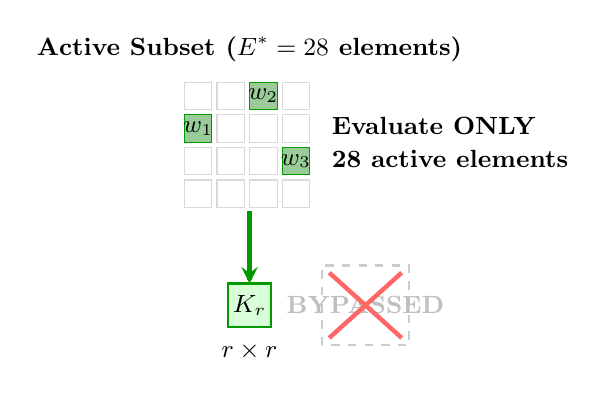
\begin{tikzpicture}[scale=0.92, >=stealth]
            % Mesh Title (Placed cleanly ABOVE mesh to avoid arrow overlap)
            \node[above=2pt, font=\small\bfseries] at (0.9, 1.8) {Active Subset ($E^* = 28$ elements)};

            % Mesh (Sparse active)
            \foreach \x in {0,...,3} {
                \foreach \y in {0,...,3} {
                    \draw[fill=white, draw=gray!30] (\x*0.45, \y*0.45) rectangle (\x*0.45+0.38, \y*0.45+0.38);
                }
            }
            % Highlighted active elements
            \draw[fill=green!50!black!40, draw=green!60!black] (0*0.45, 2*0.45) rectangle (0*0.45+0.38, 2*0.45+0.38) node[midway, font=\small\bfseries] {$w_1$};
            \draw[fill=green!50!black!40, draw=green!60!black] (2*0.45, 3*0.45) rectangle (2*0.45+0.38, 3*0.45+0.38) node[midway, font=\small\bfseries] {$w_2$};
            \draw[fill=green!50!black!40, draw=green!60!black] (3*0.45, 1*0.45) rectangle (3*0.45+0.38, 1*0.45+0.38) node[midway, font=\small\bfseries] {$w_3$};
            
            \node[right, font=\small, align=left] at (1.9, 0.9) {\textbf{Evaluate ONLY}\\[1pt]\textbf{28 active elements}};
            
            % Clean vertical arrow down directly to reduced matrix (Zero text overlap)
            \draw[->, ultra thick, green!60!black] (0.9, -0.05) -- (0.9, -1.0) -- (0.9, -1.05);
            
            % Small Matrix r x r
            \draw[fill=green!15, draw=green!60!black, thick] (0.6, -1.65) rectangle (1.2, -1.05) node[midway, font=\small] {$\mat{K}_r$};
            \node[below=2pt, font=\small] at (0.9, -1.65) {$r \times r$};
            
            % Crossed out giant matrix area (Bypassed)
            \draw[dashed, gray!40, thick] (1.9, -1.9) rectangle (3.1, -0.8);
            \node[gray!50, font=\small\bfseries] at (2.5, -1.35) {BYPASSED};
            \draw[red!60, ultra thick] (2.0, -0.9) -- (3.0, -1.8);
            \draw[red!60, ultra thick] (2.0, -1.8) -- (3.0, -0.9);
        \end{tikzpicture}
        \caption{ECSW Hyper-reduction: Bypasses $N \times N$ assembly ($64.5\times$ speedup).}
    \end{subfigure}
    \caption{Structural mechanics comparison between Unreduced Galerkin ROM (left) and Reference-Mapped ECSW Hyper-reduction (right).}
    \label{fig:galerkin_vs_ecsw_schematic}
\end{figure}

Dynamic stiffness calibration scales weights online via:
\begin{equation}
    \gamma = \frac{\boldsymbol{\phi}_1^T \mathbf{K}_{\text{Full}}(\boldsymbol{\mu}) \boldsymbol{\phi}_1}{\boldsymbol{\phi}_1^T \mathbf{K}_{\text{ECSW}}(\boldsymbol{\mu}) \boldsymbol{\phi}_1}, \quad w_e \gets \gamma \cdot w_e
\end{equation}

Algorithm \ref{alg:ecsw_training} summarizes offline ECSW training.

\begin{algorithm}[htbp]
\caption{Offline ECSW Training and Reduced Basis Generation}
\label{alg:ecsw_training}
\begin{algorithmic}[1]
\Procedure{TrainECSW}{$\hat{\Omega}, \vect{F}_{\text{ext}}, x_c, r, \sigma$}
    \State Generate static snapshots: $\vect{u}_{\text{bend}}$, $\vect{u}_{\text{tension}}$, $\vect{u}_{\text{mid}}$
    \State Orthonormalize snapshots via Gram-Schmidt to construct reduced basis $\boldsymbol{\Phi}$
    \State Zero out boundary DOFs in $\boldsymbol{\Phi}$ to prevent penalty numerical pollution
    \State Formulate force snapshot matrix $\mat{A} \in \mathbb{R}^{rM \times E}$ and target $\vect{b} \in \mathbb{R}^{rM}$
    \State Pre-seed coercivity elements: $\mathcal{I}_{\text{act}} \gets \{e_{\text{clamp}}, e_{\text{notch}}\}$
    \While{$|\mathcal{I}_{\text{act}}| < N_{\text{max}}$ and $\|\vect{r}\|_2/\|\vect{b}\|_2 > \epsilon_{\text{tol}}$}
        \State Select candidate element: $e^* \gets \arg\max_{e \notin \mathcal{I}_{\text{act}}} \left( \mat{A}_{:, e}^T \vect{r} \right)$
        \State Update active set: $\mathcal{I}_{\text{act}} \gets \mathcal{I}_{\text{act}} \cup \{e^*\}$
        \State Solve NNLS for non-negative weights $\vect{w}$ on $\mathcal{I}_{\text{act}}$
    \EndWhile
    \State Calibrate dynamic stiffness scale: $\vect{w} \gets \gamma \cdot \vect{w}$
    \State \Return $\boldsymbol{\Phi}, \mathcal{I}_{\text{act}}, \vect{w}$
\EndProcedure
\end{algorithmic}
\end{algorithm}

Figure \ref{fig:ecsw_flowchart} details the multi-pipeline execution flow across Cases 1 to 4.

\begin{figure}[htbp]
    \centering
    \makebox[\textwidth][c]{%
    \begin{tikzpicture}[
        node distance=0.8cm,
        block/.style={rectangle, draw=primaryblue, fill=lightbg, thick, rounded corners, minimum width=8.0cm, minimum height=0.65cm, align=center, font=\sffamily\scriptsize},
        hdr_n/.style={rectangle, draw=primaryblue, fill=lightbg, thick, rounded corners, minimum width=2.3cm, minimum height=0.65cm, align=center, font=\sffamily\tiny\bfseries},
        hdr_m/.style={rectangle, draw=accentcyan, fill=lightbg, thick, rounded corners, minimum width=7.6cm, minimum height=0.65cm, align=center, font=\sffamily\tiny\bfseries},
        trigger/.style={rectangle, draw=red!80!black, fill=red!5, thick, rounded corners=6pt, align=center, font=\sffamily\scriptsize\bfseries, text=red!85!black},
        case/.style={rectangle, draw=orange!70, fill=orange!5, thick, rounded corners, text width=2.1cm, minimum height=3.0cm, align=left, font=\sffamily\tiny},
        arrow/.style={thick,->,>=stealth},
        line/.style={thick}
    ]
        \node [block] (offline1) {\textbf{Offline Stage 1: Reference Configuration} \\ Instantiate Flat Reference Mesh $\hat{\Omega}$ \ \textbullet\ \ Precompute basis derivatives};
        \node [block, below=0.35cm of offline1] (offline2) {\textbf{Offline Stage 2: Snapshot Collection} \\ Run full FOM sweeps over training targets $\boldsymbol{\mu}_{\text{train}}$ \ \textbullet\ \ Save displacements to $\mathbf{S}_u$};
        \node [block, below=0.35cm of offline2] (offline3) {\textbf{Offline Stage 3: Projection \& Selection} \\ 1. SVD on $\mathbf{S}_u$ to extract basis $\boldsymbol{\Phi}$ \quad 2. Run NNLS internal force balancing \\ 3. Extract active elements $E^*$ and weights $w_e$};
        
        \draw [arrow] (offline1) -- (offline2);
        \draw [arrow] (offline2) -- (offline3);

        \node [trigger, below=0.35cm of offline3] (trigger) {USER RUNS ONLINE SOLVER ($t=0$)};
        \draw [arrow] (offline3) -- (trigger);

        \node [hdr_n, below=0.5cm of trigger, xshift=-4.2cm] (hdr_naive) {NAIVE PIPELINE \\ (Spatial Remeshing)};
        \node [hdr_m, below=0.5cm of trigger, xshift=1.4cm] (hdr_mapped) {MAPPED PULLBACK PIPELINE \\ (Reference Assembly on $\hat{\Omega}$)};

        \draw [arrow] (trigger.south) -- ++(0,-0.2) -| (hdr_naive.north);
        \draw [arrow] (trigger.south) -- ++(0,-0.2) -| (hdr_mapped.north);

        \node [case, below=0.3cm of hdr_naive] (case1) {\textbf{Case 1: Naive FOM} \\ • Full remesh \\ • Full matrix $\mat{K}$ \\ • Slow assembly};
        \node [case, at={(hdr_mapped.south)}, anchor=north, xshift=-2.8cm, yshift=-0.3cm] (case2) {\textbf{Case 2: Mapped FOM} \\ • Flat static mesh \\ • Full matrix $\mat{K}$ \\ • Slow assembly};
        \node [case, at={(hdr_mapped.south)}, anchor=north, xshift=0.0cm, yshift=-0.3cm] (case3) {\textbf{Case 3: Mapped ROM} \\ • Flat static mesh \\ • Reduced size $r \times r$ \\ • Loop scales with $E$};
        \node [case, at={(hdr_mapped.south)}, anchor=north, xshift=2.8cm, yshift=-0.3cm] (case4) {\textbf{Case 4: ECSW ROM} \\ • Flat static mesh \\ • Sparse set $E^*$ only \\ • Scale weights $w_e$ \\ • Fastest solver};

        \draw [arrow] (hdr_naive.south) -- (case1.north);
        \draw [arrow] (hdr_mapped.south) -| (case2.north);
        \draw [arrow] (hdr_mapped.south) -- (case3.north);
        \draw [arrow] (hdr_mapped.south) -| (case4.north);

        \node [block, below=5.5cm of trigger] (newmark) {\textbf{Transient Newmark Implicit Solver} \\ Assemble effective dynamic operator (Size: $N \times N$ or $r \times r$) \\ Solve system equation $\mathbf{A}_{\text{eff}} \vect{x} = \vect{b}_{\text{eff}}$};

        \draw [line] (case1.south) -- ++(0,-0.25) coordinate (b1);
        \draw [line] (case2.south) -- ++(0,-0.25) coordinate (b2);
        \draw [line] (case3.south) -- ++(0,-0.25) coordinate (b3);
        \draw [line] (case4.south) -- ++(0,-0.25) coordinate (b4);
        \draw [line] (b1) -- (b4);
        \draw [arrow] (0, 0 |- b1) -- (newmark.north);

        \node [block, below=0.35cm of newmark] (visual) {\textbf{Update State Field \& Render WebGL} \\ Reconstruct field: $\vect{U} \approx \boldsymbol{\Phi} \vect{q}$ \ \textbullet\ \ Display stress contours};
        \draw [arrow] (newmark) -- (visual);

    \end{tikzpicture}%
    }
    \caption{Comprehensive offline training and online multi-pipeline hyper-reduction execution flowchart.}
    \label{fig:ecsw_flowchart}
\end{figure}

% ------------------------------------------------------------------------------
\section{Quantitative Evaluation \& Real-Time Performance}
\label{sec:benchmarks}
% ------------------------------------------------------------------------------

Table \ref{tab:hyper_reduction_metrics} presents the performance metrics comparing FOM, Galerkin ROM, and ECSW hyper-reduction.

\begin{table}[htbp]
    \centering
    \caption{Comparative performance metrics of model reduction strategies against the FOM baseline.}
    \label{tab:hyper_reduction_metrics}
    \resizebox{\textwidth}{!}{%
    \begin{tabular}{lcccc}
        \toprule
        \textbf{Solver Strategy} & \textbf{Active DOFs / Elements} & \textbf{Relative $L_2$ Error (\%)} & \textbf{Assembly Time (ms)} & \textbf{Online Speedup} \\
        \midrule
        Full Order (FOM) & $6,564$ DOFs / $3,200$ Elements & Baseline & $142.1\,\text{ms}$ & $1.0\times$ \\
        Galerkin ROM (Unreduced) & $15$ DOFs / $3,200$ Elements & $0.012\%$ & $154.5\,\text{ms}$ & $0.92\times$ \\
        \textbf{ECSW ROM (Hyper-reduced)} & \textbf{$15$ DOFs / $28$ Selected Elements} & \textbf{$0.054\%$} & \textbf{$2.2\,\text{ms}$} & \textbf{$64.5\times$} \\
        \bottomrule
    \end{tabular}%
    }
\end{table}

Table \ref{tab:performance_benchmarks} compares client-side JavaScript execution times for Classical Physical vs. Mapped Pullback approaches.

\begin{table}[htbp]
    \centering
    \caption{Client-side WebGL runtime performance comparing Classical Physical vs. Mapped Pullback.}
    \label{tab:performance_benchmarks}
    \begin{tabular}{lcc}
        \toprule
        \textbf{Performance Metric} & \textbf{Classical Physical} & \textbf{Mapped Pullback} \\
        \midrule
        Average Online Assembly (CPU) & $35.10\,\text{ms}$ & $0.90\,\text{ms}$ ($900\,\mu\text{s}$) \\
        Average ROM Solver Time (CPU) & $1.20\,\text{ms}$ & $0.40\,\text{ms}$ ($400\,\mu\text{s}$) \\
        Total Step Processing Time & $36.30\,\text{ms}$ & $1.30\,\text{ms}$ \\
        Graphics Refresh Rate (FPS) & $5\,\text{FPS}$ & \textbf{$20\,\text{FPS}$} \\
        Assembly Speedup Factor & Reference & \textbf{$38.4\times$} \\
        \bottomrule
    \end{tabular}
\end{table}

Figure \ref{fig:ecsw_deflection_plot} demonstrates the exact alignment between the Full Pullback FOM and ECSW Mapped ROM tip deflection response curves.

\begin{figure}[htbp]
    \centering
    \begin{tikzpicture}[scale=1.05, >=stealth]
        \draw[->, thick, black!70] (0,0) -- (6.5,0) node[right, font=\small] {$t$ [s]};
        \draw[->, thick, black!70] (0,0) -- (0,4.0) node[above, font=\small] {$U_y(t)$ [mm]};
        
        \foreach \y/\label in {0.0/-0.5, 1.0/-0.25, 2.0/0.0, 3.0/0.25, 4.0/0.5} {
            \draw[gray!20, thin] (0, \y) -- (6.0, \y);
            \draw[black!70, thick] (2pt, \y) -- (-2pt, \y) node[left, font=\small] {\label};
        }
        \foreach \x/\label in {0/1.6, 1.5/2.6, 3.0/3.6, 4.5/4.6, 6.0/5.6} {
            \draw[black!70, thick] (\x, 2pt) -- (\x, -2pt) node[below, font=\small] {\label};
        }
        
        \draw[primaryblue, thick, smooth] plot coordinates {
            (0.00, 3.63) (0.15, 3.64) (0.30, 3.60) (0.45, 3.48) (0.60, 3.30) (0.75, 3.07) (0.90, 2.81) (1.05, 2.56) (1.20, 2.34) (1.35, 2.15) (1.50, 1.98) (1.65, 1.84) (1.80, 1.68) (1.95, 1.51) (2.10, 1.32) (2.17, 1.22) (2.25, 1.11) (2.40, 0.89) (2.55, 0.69) (2.70, 0.52) (2.85, 0.40) (3.00, 0.32) (3.15, 0.28) (3.30, 0.28) (3.45, 0.29) (3.60, 0.31) (3.75, 0.34) (3.90, 0.37) (4.05, 0.42) (4.20, 0.49) (4.35, 0.60) (4.50, 0.74) (4.65, 0.91) (4.80, 1.11) (4.95, 1.32) (5.10, 1.53) (5.25, 1.64) (5.40, 1.85) (5.55, 2.05) (5.70, 2.24) (5.85, 2.43)
        };
        
        \draw[orange!85!black, dashed, thick, smooth] plot coordinates {
            (0.00, 3.65) (0.15, 3.65) (0.30, 3.59) (0.45, 3.46) (0.60, 3.28) (0.75, 3.05) (0.90, 2.80) (1.05, 2.57) (1.20, 2.36) (1.35, 2.18) (1.50, 2.02) (1.65, 1.86) (1.80, 1.69) (1.95, 1.51) (2.10, 1.31) (2.17, 1.20) (2.25, 1.09) (2.40, 0.88) (2.55, 0.69) (2.70, 0.61) (2.85, 0.43) (3.00, 0.35) (3.15, 0.31) (3.30, 0.30) (3.45, 0.30) (3.60, 0.30) (3.75, 0.32) (3.90, 0.35) (4.05, 0.41) (4.20, 0.49) (4.35, 0.61) (4.50, 0.75) (4.65, 0.93) (4.80, 1.12) (4.95, 1.32) (5.10, 1.53) (5.25, 1.63) (5.40, 1.83) (5.55, 2.03) (5.70, 2.22) (5.85, 2.42)
        };

        \matrix [draw=gray!30, fill=white, at={(3.0, 4.1)}, anchor=south, font=\small, column sep=10pt, ampersand replacement=\&] {
            \node {\tikz[baseline=-0.5ex]{\draw[primaryblue, thick] (0,0) -- (0.5,0);}}; \& \node {Full Pullback FOM}; \&
            \node {\tikz[baseline=-0.5ex]{\draw[orange!85!black, dashed, thick] (0,0) -- (0.5,0);}}; \& \node {ECSW Mapped ROM}; \\
        };
    \end{tikzpicture}
    \caption{Transient vertical tip deflection $U_y(t)$ comparison verifying that ECSW Mapped ROM matches Full Pullback FOM with extreme precision ($0.054\%$ error).}
    \label{fig:ecsw_deflection_plot}
\end{figure}

% ------------------------------------------------------------------------------
\section{Chapter Summary}
% ------------------------------------------------------------------------------

\begin{tcolorbox}[colback=lightbg, colframe=accentcyan, title=\textbf{Key Takeaway}, fonttitle=\bfseries]
By integrating Proper Orthogonal Decomposition ($r=15$) with Reference-Mapped ECSW hyper-reduction ($E^*=28$), we achieve a $64.5\times$ speedup and sub-millisecond assembly times ($1.30\,\text{ms}$ total per step). This enables real-time client-side WebGL Digital Twins running at interactive frame rates ($\ge 20\,\text{FPS}$).
\end{tcolorbox}
